\documentclass[runningheads,a4paper]{llncs}
\usepackage{cite}
\usepackage{graphicx}
\usepackage{listings}
 
%-------------------------------------------------
% Comments/Collaboration
%-------------------------------------------------
\usepackage[dvipsnames]{xcolor}
\usepackage{todonotes}
\newcommand\will[1]{\todo[author=Will,color=Orchid]{#1}}
\newcommand\tim[1]{\todo[author=Tim,color=Apricot]{#1}}
\newcommand\richard[1]{\todo[author=Richard,color=JungleGreen]{#1}}

\authorrunning{Ran Wei, Tim P. Kelly, Richard Hawkins}

\makeatletter
\renewcommand\subsubsection{\@startsection{subsubsection}{3}{\z@}%
	{-18\p@ \@plus -4\p@ \@minus -4\p@}%
	{4\p@ \@plus 2\p@ \@minus 2\p@}%
	{\normalfont\normalsize\bfseries\boldmath
		\rightskip=\z@ \@plus 8em\pretolerance=10000 }}
\renewcommand\paragraph{\@startsection{paragraph}{4}{\z@}%
	{-12\p@ \@plus -4\p@ \@minus -4\p@}%
	{2\p@ \@plus 1\p@ \@minus 1\p@}%
	{\normalfont\normalsize\itshape
		\rightskip=\z@ \@plus 8em\pretolerance=10000 }}
\makeatother




\begin{document}
 
\title{\textbf{A Systematic Approach For Model Based System Assurance}}
\author{Ran Wei \and Tim P. Kelly \and Richard Hawkins}
\institute{University of York, United Kingdom 
\email{\{ran.wei,tim.kelly,richard.hawkins\}@york.ac.uk}
}
\maketitle

\begin{abstract}
Assurance cases are used to demonstrate confidence in properties of interest for a system, e.g. for safety or security. Typically, the task of constructing assurance cases is a lengthy and informal process. In recent years, there has been work to propose model based approaches to promote automation. The Structured Assurance Case Metamodel (SACM) is an OMG specification designed to represent system assurances in machine-readable models, so that a series of model management operations can be 
performed to automate the process of system assurance. However, the adoption of SACM faces challenges as there is a cognitive gap between the syntax/semantics of SACM elements and system assurance practitioners' understanding of SACM.

In this paper, we provide a definitive guide to SACM with examples so that SACM can be better understood. We also discuss the relationship between SACM and the Goal Structuring Notation (GSN) and the interoperability between them. We also propose a systematic approach for model based system assurance using SACM, so that all corresponding models can be bridged together using the facilities provided in SACM.
\end{abstract}


\section{Introduction}

\section{Structured Assurance Case Metamodel}

\section{Structured Assurance Case Metamodel and the Goal Structuring Notation}

\begin{figure}
	\centering
	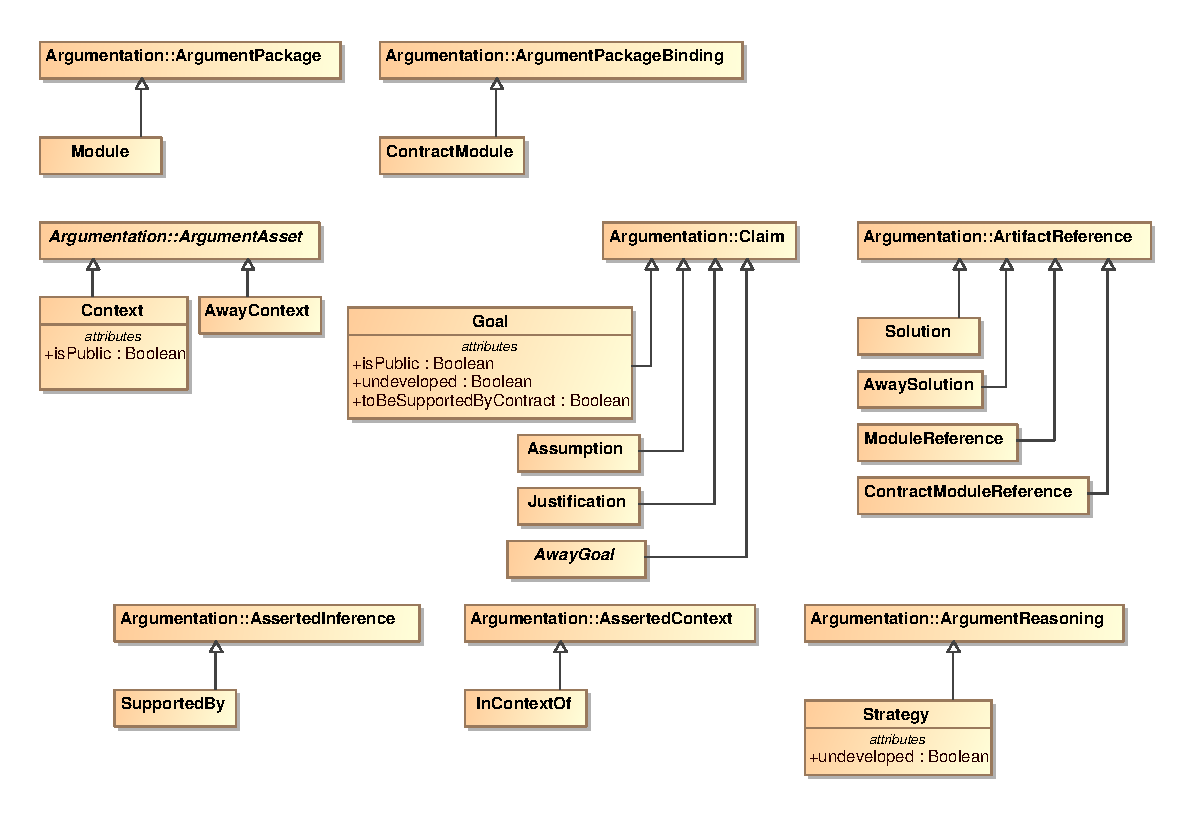
\includegraphics[width=1\linewidth]{GSNMetamodel.eps}
	\caption{An \textbf{asCited} \textit{Claim}.}
	\label{fig:asCitedClaim}
\end{figure}

\section{Running example: a systematic approach}

\section{Tool Support and Related Work}

\section{Conclusion}

Safety Case Construction
and Reuse using Patterns

\noindent\textbf{Acknowledgements}
This work is supported by the European Union'’s Horizon 2020 research and innovation programme through the DEIS project (grant agreement No 732242). 

\bibliographystyle{unsrt} 
\bibliography{references}  

\end{document}
